% CF-Verify — ACL/ARR submission version (converted from LNCS)
% Body ≤ 8 pages (review mode); unlimited appendix (limitations onward).
\documentclass[11pt]{article}

\usepackage[review]{acl}
\usepackage{times}
\usepackage{latexsym}
\usepackage[T1]{fontenc}
\usepackage[utf8]{inputenc}
\usepackage{microtype}
\usepackage{inconsolata}
\usepackage{graphicx}
\usepackage{booktabs}
\usepackage{amsmath}
\usepackage{amssymb}
\usepackage{multirow}
\usepackage{url}
\usepackage{caption}

\title{CF-Verify: Counterfactual Evidence Deletion as a Behavioural\\Evidence-Dependence Diagnostic for Retrieval-Augmented Multi-Hop QA}

\author{Anonymous Author(s) \\ Anonymous Institution \\ \texttt{anonymous@example.org}}

\begin{document}
% Force US Letter page size (ACL/ARR requirement)
\pdfpagewidth=8.5in
\pdfpageheight=11in

\maketitle

\begin{abstract}
For a RAG agent, an answer can be topically \emph{compatible} with retrieved text yet produced entirely from parametric memory. We separate evidence \emph{compatibility} from \emph{behavioural evidence dependence}, that is, whether the model would change its answer if the evidence were removed. We introduce \textbf{CF-Verify}, a training-free, black-box diagnostic that has the LLM answer with full evidence, marks the sentences a self-rationale pass relied on, deletes only those sentences, re-answers, and compares the change against a matched random-deletion baseline, yielding a CFScore for accept / revise / re-retrieve decisions. Across three multi-hop benchmarks (HotpotQA, 2WikiMultihopQA, MuSiQue) and five models (GPT-5.4, GPT-5.4-mini, GPT-5.5, Mistral-7B, Llama-3.1-8B), the pooled GPT-5.4 CFScore over 321 answered questions is $+0.657$ (95\% CI $[+0.601, +0.713]$), and on a 300-question grounded/ungrounded paired benchmark CF-Verify reaches AUROC 0.784 versus 0.533 for an LLM-judge and 0.664 for a BGE-similarity baseline.
\end{abstract}

\section{Introduction}
\label{sec:intro}

Retrieval-augmented generation (RAG) is increasingly used in question answering systems that must answer from external evidence rather than from the model's parametric memory. This requirement is especially important in multi-hop QA, where the answer combines facts scattered across several passages. A confident-looking answer, however, is not necessarily an evidence-grounded answer: the model may produce the correct response because retrieved passages support it, or because the answer was already memorized during pre-training. For downstream decisions, these two cases should be treated differently. Figure~\ref{fig:concept} organizes this distinction as a 2$\times$2: whether the answer is \emph{compatible} with the evidence (a property judges already check) versus whether it \emph{behaviourally depends} on the evidence (the property CF-Verify tests).

\begin{figure}[htbp]
    \centering
    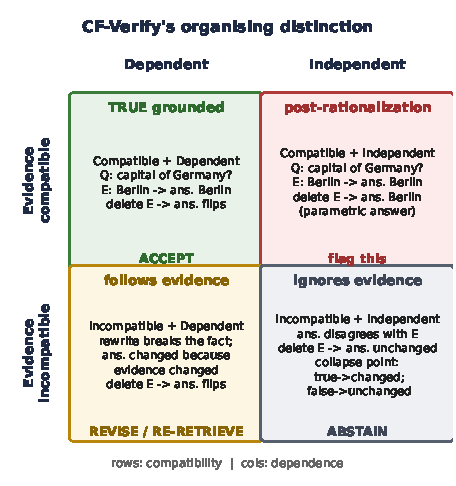
\includegraphics[width=\columnwidth]{figures/concept_2x2.pdf}
    \caption{The organizing distinction of this paper: \emph{evidence compatibility} (top row: the answer is topically consistent with the retrieved evidence) is not \emph{behavioural evidence dependence} (the answer changes when the evidence is deleted). Only the behavioural test separates the true-grounded case (top-left) from post-rationalization of a parametric answer (top-right), the case that compatibility-based judges, including LLM-as-judge, systematically miss. CF-Verify routes each quadrant: ACCEPT, REVISE/RE-RETRIEVE, or ABSTAIN.}
    \label{fig:concept}
\end{figure}

We therefore study \emph{grounding verification} for retrieval-augmented multi-hop QA. The goal is not to judge whether an answer is factually correct in the world, but to determine whether the answer is \emph{behaviourally supported} by the retrieved evidence used in the current interaction. This distinction matters for system control: if an answer is grounded, the agent can accept it with higher confidence; if it is ungrounded, the agent may need to revise, retrieve additional evidence, or abstain.

We propose \textbf{CF-Verify}, a counterfactual verification method based on evidence deletion. Given a question, retrieved context, and model answer, CF-Verify runs the same language model twice: once with the full evidence and once with predicted supporting sentences removed. If the answer changes under this targeted intervention, the original answer depended on those sentences. To rule out generic prompt-perturbation noise, we compare the targeted flip rate against a \emph{matched random-deletion} baseline and use the difference, the \textbf{CFScore}, as the evidence-dependence signal. The score yields a three-way accept/revise/re-retrieve decision.

Three challenges shape the design. First, existing signals (confidence, retrieval similarity, answer--context overlap) are correlational: a model can assign high confidence to an answer recoverable from parametric memory, and a retrieved passage can lexically overlap the answer without being necessary. CF-Verify formulates grounding verification as a counterfactual test, so the target moves from static agreement to causal dependence in model behaviour. Second, removing arbitrary text can alter output simply because the prompt changed. The matched random-deletion baseline normalizes this away; the remaining effect is attributed to the removed support. Under gold annotations CF-Verify achieves a headline CFScore of $0.93$ ($94.7\%$ targeted vs.\ $1.8\%$ random flips); the larger-scale pooled estimate is $+0.657$ (95\% CI $[+0.601, +0.713]$). Third, a practical method must not depend on labelled supporting sentences. A self-rationale variant predicts the support set automatically and retains a CFScore of $0.81$ on the pilot sample.

Our contributions:
\begin{itemize}\itemsep0pt
\item \textbf{C1.} A training-free, black-box counterfactual evidence-dependence test (CFScore = targeted flip rate $-$ matched random flip rate) with a three-way routing rule for RAG agents.
\item \textbf{C2.} A large-scale empirical characterization: three multi-hop benchmarks, five models spanning proprietary and open weights (GPT-5.4/5.4-mini/5.5, Mistral-7B, Llama-3.1-8B), pooled GPT-5.4 CFScore $+0.657$ over 321 answered questions.
\item \textbf{C3.} A 300-question grounded/ungrounded paired benchmark with verifier baselines: CF-Verify (AUROC 0.784 curated; 0.656 unconditional at scale) beats an LLM-judge (0.533) and BGE similarity (0.664); a content-matched random control and a 2D rewrite-validity $\times$ evidence-sensitivity stratification show the discrimination is concentrated on evidence-sensitive questions (clean quadrant AUROC 0.762).
\item \textbf{C4.} Honest negative results: a merged-prompt cost variant collapses on Mistral-7B via a calibration mechanism we diagnose (abstention suppression), and unconditional detection degrades when questions are parametrically answerable; together these define the applicability boundary of behavioural verification.
\end{itemize}

\section{Related Work}
\label{sec:related}

\paragraph{Faithfulness and factuality evaluation.}
SelfCheckGPT \cite{selfcheckgpt} estimates factuality from sampled-response consistency; FactScore \cite{factscore} decomposes long-form generation into atomic claims and checks each against evidence; RARR \cite{rarr} retrieves and revises outputs for attribution; RAGAS \cite{ragas} provides reference-free RAG metrics; recent judge-based benchmarks \cite{tamber2025faithjudge} systematize hallucination evaluation. These methods frame verification as a judgement task: an evaluator LLM decides whether an answer is supported. But judgement alone is insufficient. The judge and the generator share parametric knowledge, biases, and failure modes, so a second opinion can re-introduce the hallucination it was meant to detect. CF-Verify intervenes on the evidence and observes whether the same model changes its answer. The core signal is counterfactual sensitivity, not a second opinion.

\paragraph{Grounding, citation, and attribution in RAG.}
Knowledge-conflict work trains, edits, or constrains the generator so that it \emph{prefers} retrieved context over parametric memory: context-faithful decoding, hidden-state rectification, contrastive training, and copy-oriented generation \cite{zhao2026guarantrag,ma2026corect,tan2026ctrlrag,long2026copypastellm} each push the model to rely more on retrieved text. These methods act on the generation process and need training, internal access, or modified decoding. We address a different problem: \emph{verifying}, after the fact, that the model did rely on the evidence. CF-Verify is a post-hoc, black-box verification layer, complementary to the generation-time interventions above.

\paragraph{Counterfactual attribution.}
We separate \emph{offline attribution} (scoring which evidence plausibly explains an answer) from \emph{online verification} (deciding at deployment time whether an answer can be trusted as evidence-dependent). Closest to our setting, \citet{saharoy2024counterfactual} apply removal-based counterfactual attribution in RAG over heterogeneous data, and \citet{wallat2024correctness} audit whether cited evidence genuinely supports the answer or is post-rationalised; both produce post-hoc scores for analysis. CF-Verify differs from both in three ways: \textbf{(i) black-box vs.\ internal} (no attention, hidden states, or surrogates); \textbf{(ii) differential vs.\ pointwise} (CFScore subtracts a matched random-deletion baseline that prior attribution scores lack); \textbf{(iii) operational vs.\ post-hoc} (CF-Verify emits an accept/revise/re-retrieve decision rather than an offline attribution score).

\section{Method}
\label{sec:method}

\begin{figure*}[htbp]
    \centering
    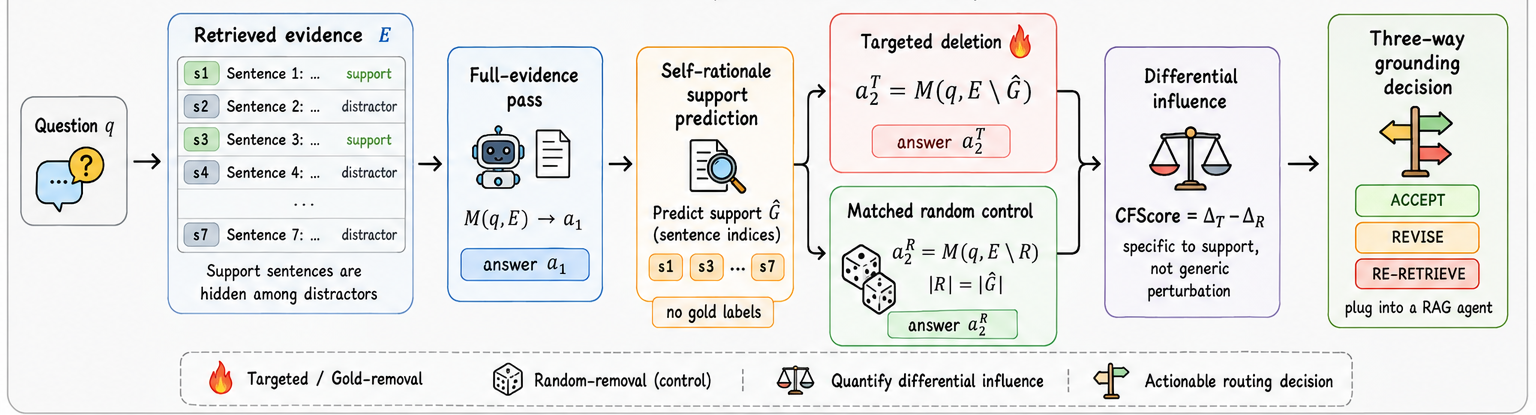
\includegraphics[width=\linewidth]{figures/fig_main.png}
    \caption{Overview of the CF-Verify pipeline: (i) self-rationale support prediction $\hat{G}$, (ii) targeted deletion ($E\setminus\hat{G}$) and matched random deletion ($E\setminus R$), (iii) differential score $\mathrm{CFScore} = \widehat{F_T}-\widehat{F_R}$, (iv) three-way routing.}
    \label{fig:main}
\end{figure*}

\subsection{Problem Formulation}
We start with a question $q$, retrieved evidence sentences $E=\{s_1,\dots,s_n\}$, and a black-box LLM $M$. The agent produces an answer $a^{(0)} = M(q, E)$. A \emph{support set} $G \subseteq E$ is the subset whose removal would change the answer. We frame verification as a question about behavioural dependence: does $a^{(0)}$ depend on the candidate support $\hat{G}$?

\subsection{Targeted Counterfactual Deletion}
We prompt $M$ with a self-rationale template that asks it to list the indices of evidence sentences it actually used; this yields the predicted support $\hat{G}$. We then remove $\hat{G}$ from the prompt:
\begin{equation}
E^{-\hat{G}} = E \setminus \hat{G}, \qquad a^{(1)} = M(q, E^{-\hat{G}}).
\end{equation}
The targeted flip indicator $\phi_T(q,E) = \mathbb{1}[a^{(1)} \neq a^{(0)}]$ (under an answer-equivalence function $\Delta$) captures whether the model still answers the same way once $\hat{G}$ is gone, isolating evidence dependence from prompt noise.

\subsection{Matched Random-Deletion Control}
Removing any text perturbs the prompt; a flip may reflect formatting or length effects rather than lost support. CF-Verify therefore samples a control set
\begin{equation}
R \sim \mathcal{U}\big(\{R' \subseteq E\setminus\hat{G} : |R'| = |\hat{G}|\}\big),
\end{equation}
matched to $\hat{G}$ on three axes: \textbf{(i)} matched on size, \textbf{(ii)} drawn from the same source, and \textbf{(iii)} disjoint from the predicted support $\hat{G}$. The controls cancel the features known to drive prompt-perturbation noise without begging the question of content relevance. We estimate the random flip indicator $\phi_R$ with $K$ independent samples.

\subsection{CFScore and Routing}
\begin{equation}
\mathrm{CFScore}(q,E) = \widehat{F_T} - \widehat{F_R}, \qquad \mathrm{CFScore} \in [-1,1].
\end{equation}
The CFScore measures how much more the answer depends on the targeted support than on equally-sized random text, so high values mean evidence genuinely drove the answer. We ACCEPT when CFScore $\geq \tau$ (the answer behaviourally depends on the predicted support); RE-RETRIEVE when $\widehat{F_T}$ is high but evidence is judged insufficient; REVISE otherwise. We fix $\tau = 0.5$ throughout and report threshold sensitivity in Appendix~\ref{app:threshold}.

\section{Experiments}
\label{sec:exp}

\subsection{Setup}
We examine behavioural evidence dependence of LLM answers along four axes. (i)~\emph{Corpus-level estimation}: CFScore at scale on HotpotQA distractor \cite{hotpotqa}, 2WikiMultihopQA, and MuSiQue \cite{2wikimultihopqa} dev splits, with $617$ attempted questions pooled. We test whether targeted deletion flips answers where matched random deletion does not. (ii)~\emph{Grounded/ungrounded paired detection}: 60 paired records per question (gold support kept vs.\ fact-breaking rewrites); we test whether CFScore separates the two conditions better than similarity or judge baselines. (iii)~\emph{Conditional validity at scale}: extension of the paired benchmark to $N{=}300$ with stratification by evidence sensitivity and rewrite validity, to map where behavioural verification applies. (iv)~\emph{Model-capability boundary}: five models probed (GPT-5.4 (primary, via API), GPT-5.4-mini, GPT-5.5, Mistral-7B-Instruct-v0.3, and Llama-3.1-8B-Instruct), plus two protocol repairs, to separate model failures from measurement artifacts. The headline protocol uses gold support annotations, $K{=}1$; the detection analyses use $K{=}5$. Exact-match $\Delta$ is the default; a BGE semantic $\Delta$ is reported as a robustness check (Appendix~\ref{app:semantic}).

\subsection{Corpus-Level Evidence Dependence}
\label{sec:headline}
\begin{figure}[htbp]
    \centering
    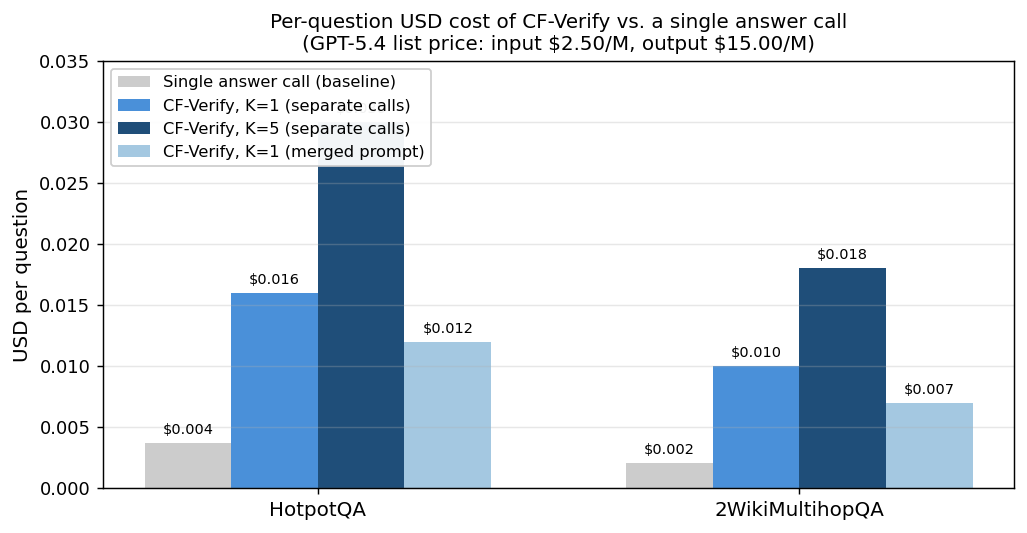
\includegraphics[width=0.95\linewidth]{figures/cost_breakdown.png}
    \caption{Per-question USD cost of CF-Verify vs.\ a single answer call (GPT-5.4 list price). At $K{=}1$ CF-Verify is a $\sim$$4\times$ multiplier on per-query inference cost; the merged prompt saves $\sim$25\% on capable models.}
    \label{fig:cost}
\end{figure}
We ask whether targeted deletion flips answers where matched random deletion does not. Table~\ref{tab:multimodel} answers yes, across all five models and three datasets. On the curated headline sample ($N{=}57$), targeted deletion flips $94.7\%$ of answers vs.\ $1.8\%$ under matched random deletion. On the full pooled sample, per-dataset CFScores are HotpotQA $+0.603$, 2Wiki $+0.806$, MuSiQue $+0.711$ (10{,}000-resample bootstrap CIs $[+0.533,+0.673]$, $[+0.694,+0.903]$, $[+0.578,+0.844]$). The headline value was a high outlier; the pooled estimate is the more reliable one and still a $4.6\times$ multiplier over the random baseline. A worst-case selection-bias analysis treating abstentions as flips on both arms yields CFScore $+0.329$, still positive (Appendix~\ref{app:selection}).

\begin{table*}[t]
\centering
\small
\caption{Multi-model and multi-dataset CFScore (gold supports, $K{=}1$, answered subset). ``Answered'' = substantive full-evidence answer; rates over the answered subset.}
\label{tab:multimodel}
\begin{tabular}{@{}lcccc@{}}
\toprule
Setting & $N$ & Answered & $\widehat{F_T}$ / $\widehat{F_R}$ & CFScore \\
\midrule
GPT-5.4 headline (HotpotQA)  & 30 & 30/30 & 93.3\% / 3.3\%  & $+0.900$ \\
GPT-5.4 headline (2Wiki)     & 27 & 27/27 & 96.3\% / 0.0\%  & $+0.963$ \\
GPT-5.4-mini (60 Q pool)     & 60 & 52/60 & 84.6\% / 19.2\% & $+0.654$ \\
GPT-5.5 (60 Q pool)          & 60 & 53/60 & 79.2\% / 17.0\% & $+0.623$ \\
Llama-3.1-8B-Instruct        & 60 & 36/60 & 94.4\% / 13.9\% & $+0.806$ \\
Mistral-7B (separate calls)  & 60 & 14/60 & 64.3\% / 0.0\%  & $+0.643$ \\
\midrule
GPT-5.4 larger sample III (qid 71--280) & 420 & 145/420 & 69.0\% / 15.2\% & $+0.538$ \\
GPT-5.4 MuSiQue              & 60 & 45/60 & 100\% / 28.9\%  & $+0.711$ \\
\midrule
\textbf{GPT-5.4 pooled, all three datasets} & \textbf{321} & \textbf{321/617} & \textbf{80.8\% / 14.5\%} & $\mathbf{+0.657}$ \\
\bottomrule
\end{tabular}
\end{table*}

\subsection{Cost and Stability}
\label{sec:cost}
We test whether the cost and variance of CF-Verify stay within operational limits. At the GPT-5.4 list price, one verification at $K{=}1$ costs $\sim$\$0.016 (HotpotQA; \$0.010 on 2Wiki), a $\sim$$4\times$ multiplier over a single answer call (Figure~\ref{fig:cost}); the merged variant saves $\sim$25\% where applicable, and triggering verification only on low-confidence items amortises it further. The headline estimate is stable: a 10{,}000-resample bootstrap gives 95\% CI $[0.860, 0.982]$ on the pilot and $[+0.601,+0.713]$ pooled; leave-one-out influence is bounded by $\pm 0.017$; subsample SD converges to $0.034$ by $N{=}57$ (Figure~\ref{fig:bootstrap}).

\subsection{Grounded/Ungrounded Detection}
\label{sec:detection}
We test whether the score separates grounded from ungrounded evidence. We construct paired test cases: for each question, the gold supporting sentences are either kept (\emph{grounded}) or replaced by gpt-5.4 rewrites that preserve topic and entities but break the supporting fact (\emph{ungrounded}). A faithful model should change its answer (or abstain) on the ungrounded variant. AUROC reaches $0.784 \pm 0.013$ for CF-Verify on Table~\ref{tab:detection_all} (5-fold CV; a group-wise split by question gives $0.784 \pm 0.014$, ruling out intra-question leakage), and the logistic BGE+CFScore ensemble runs higher still at $0.804$; the two signals are complementary, not redundant. The judge's near-chance AUROC ($0.533$) is diagnostic: because ungrounded records remain topically consistent with the evidence, a judge reading for compatibility cannot separate the conditions, exactly the compatibility-vs.-dependence distinction that motivates behavioural testing.

A content-matched control addresses the strongest remaining confound: instead of uniform random deletion, we delete the $k$ non-support sentences most BGE-similar to the gold support. If CF-Verify merely detected ``deletion of answer-related text,'' this control would close the gap; instead $\widehat{F_R}$ rises only from $31.0\%$ to $38.3\%$ and CFScore stays at $+0.483$, a $48.4$-point targeted-vs-control gap, with the two deleted sets matched on length, position, and question-word overlap (Appendix~\ref{app:content}).

\paragraph{Routing utility.}
Detection can also be reframed as an accept/revise decision (ACCEPT iff the detector signals grounded; 5-fold CV with fold-internal threshold selection). Under this framing, Table~\ref{tab:detection_all} reports routing F1 against the always-ACCEPT prior of $0.667$ (precision $0.696$, recall $0.750$ for CF-Verify; $0.762/0.867$ for the ensemble). Routing F1 alone shows CF-Verify at $0.712$, BGE at $0.682$, and the ensemble at $0.809$. With 1{,}000-resample bootstrap CIs, the paired CF-vs-BGE F1 difference ($+0.025$, CI $[-0.058,+0.111]$) is not significant at 120 records. We state plainly: \emph{as a stand-alone router the advantage over a similarity baseline is not resolvable at this sample size; the significant gain comes from the ensemble}, where behavioural and similarity signals are complementary.

\begin{table}[t]
\centering
\small
\caption{Detection and routing on the curated 60-question benchmark (120 paired records, 5-fold CV).}
\label{tab:detection_all}
\begin{tabular}{@{}lcc@{}}
\toprule
Verifier & AUROC & Routing F1 \\
\midrule
LLM-as-judge (gpt-5.4) & 0.533 & -- \\
BGE sim (answer, gold)  & 0.664 & 0.682 \\
CF-Verify CFScore ($K{=}5$) & 0.784 & 0.712 \\
BGE + CF (logistic) & \textbf{0.804} & \textbf{0.809} \\
\bottomrule
\end{tabular}
\end{table}

\subsection{Scaling the Paired Benchmark: Conditional Validity}
\label{sec:conditional}
We ask whether the headline detection result holds when the paired set is extended to $N{=}300$ questions (600 records; 80 each from HotpotQA/2Wiki/MuSiQue). The unconditional AUROC drops to $0.656 \pm 0.033$ and routing F1 to $0.658$, marginally below the always-ACCEPT F1 of $0.667$. This drop is real, and stratification reveals \emph{where} behavioural verification applies (Table~\ref{tab:conditional}):

\begin{table}[t]
\centering
\small
\caption{Conditional validity on the $N{=}300$ paired benchmark. ``Sensitivity'' = targeted deletion flips the grounded answer ($\widehat{F_T}{=}1$). ``Validity'' = rewrite changed the full-evidence answer. ``No-evidence gate'' = GPT-5.4 abstains on the question when given no evidence (proxy for ``not parametrically answerable''). Always-ACCEPT F1 = 0.667.}
\label{tab:conditional}
\begin{tabular}{@{}lcc@{}}
\toprule
Subset & N & AUROC \\
\midrule
All (unconditional)            & 600 rec & $0.656{\pm}.033$ \\
Evidence-sensitive (80\%)      & 478 rec & $0.740{\pm}.037$ \\
Valid rewrite \& sensitive (62\%) & 370 rec & $\mathbf{0.762}$ \\
\midrule
No-evidence gate abstains (29\%) & 174 rec & $0.713$ \\
\bottomrule
\end{tabular}
\end{table}

The evidence-sensitive subset ($80\%$ of questions) recovers most of the headline AUROC: $0.740 \pm 0.037$, with routing F1 $0.711$ exceeding always-ACCEPT by $4.4$ points, reproduced on each dataset (HotpotQA $0.737$, 2Wiki $0.747$, MuSiQue $0.725$). The insensitive subset ($20\%$; the model answers identically with or without the support) shows AUROC of $0.336$, correctly so, since there is no behavioural dependence to detect. The clean quadrant -- valid rewrites on sensitive questions ($62\%$) -- reproduces the curated benchmark's AUROC almost exactly ($0.762$ vs.\ $0.784$), ruling out the small-sample-luck explanation. The unconditional drop is a mixture of parametrically answerable questions, on which \emph{no} behavioural verifier should be expected to work, and imperfect synthetic negatives ($32\%$ of rewrites fail to change the answer; a manual audit finds failure modes such as the rewrite retaining the answer entity). We report all quadrants (Appendix~\ref{app:2d}) and recommend the conditional framing for deployment: route through CF-Verify when a cheap evidence-sensitivity probe indicates behavioural dependence.

\subsection{Model-Capability Boundary and Two Practical Repairs}
\label{sec:merged}
We test whether the merged-prompt variant ($3{+}K \to 2{+}K$ calls, a $33\%$ saving) holds across model capabilities. Table~\ref{tab:merged} reveals a sharp split between GPT-5.4 and Mistral-7B under three repair variants. On GPT-5.4 the merged variant works: $\hat{G}$ F1 \emph{rises} to $0.835$ and CFScore stays at $+0.558$. On Mistral-7B the v1 (strict JSON parser) and v2 (lenient parser) variants give F1 $0.04$ / $0.38$ and CFScore $+0.130$ / $+0.109$, far below the separate-call baseline of $+0.643$. Two practical repairs recover much of the gap:

\textbf{(i) Format-consistent random baseline (v5).} The first four variants compared the merged call's JSON-embedded answer against random-deletion answers from a plain simple prompt. Cross-format string comparison produces spurious flips when the merged answer contains a full sentence (e.g.\ ``Eenasul Fateh, also known by his stage name Aladin'') and the simple-prompt answer is shorter. Re-running the random-deletion probes through the same merged prompt (v5) drops $\widehat{F_R}$ from $87.0\%$ to $23.3\%$ and lifts CFScore from $+0.109$ to $+0.433$. The Mistral collapse was partly a measurement artifact; the underlying model still underperforms GPT-5.4 but is within operational margin once comparisons are format-consistent.

\textbf{(ii) No-evidence parametric-answerability gate.} Across the 300-question paired benchmark we probe gpt-5.4 with the question but no evidence; the model abstains on $28.7\%$ of questions and produces a substantive answer on the remaining $71.3\%$. On the $86$ questions where the gate abstains, the subset where the question cannot be answered from parametric memory and grounding is therefore a behavioural concern, and CF-Verify's pooled CFScore recovers to $+0.595$ (Table~\ref{tab:conditional}, sensitive subset row).

\begin{table}[t]
\centering
\scriptsize
\caption{Merged-prompt variants on Mistral-7B-Instruct-v0.3. v1 (strict JSON parser), v2 (lenient parser), v3 (nullable-answer gate), v4 (two-shot in-context exemplars), v5 (this work: format-consistent random baseline).}
\label{tab:merged}
\begin{tabular}{@{}lcccc@{}}
\toprule
Setting & Ans. & $\widehat{F_T}$ & $\widehat{F_R}$ & CFScore \\
\midrule
Mistral separate (gold)   & 14/60 & 64.3\% & 0.0\%  & $+0.643$ \\
Mistral merged v1 (strict) & 46/60 & 97.8\% & 87.0\% & $+0.130$ \\
Mistral merged v2 (lenient)& 46/60 & 97.8\% & 87.0\% & $+0.109$ \\
Mistral merged v3 (nullable)& 53/60 & 100\% & 100\% & $0.000$ \\
Mistral merged v4 (2-shot) & 33/60 & 100\% & 83.8\% & $+0.162$ \\
\textbf{Mistral v5 (consistent)} & 60/60 & \textbf{66.7\%} & \textbf{23.3\%} & $\mathbf{+0.433}$ \\
\midrule
GPT-5.4 separate (gold)   & 57/57 & 94.7\% & 1.8\% & $+0.930$ \\
GPT-5.4 merged              & 52/60 & 92.3\% & 36.5\% & $+0.558$ \\
\bottomrule
\end{tabular}
\end{table}

\paragraph{Deployment guidance.} Capable models (GPT-5.4, GPT-5.5, Llama-3.1-8B) handle the merged prompt well: a third of the calls saved with a modest CFScore discount, so this is the recommended deployment default. Smaller models (Mistral-7B-class) need a format-consistent random baseline (v5) and a no-evidence parametric-answerability gate to filter the question set to one where grounding is a behavioural concern. Together these two repairs raise Mistral-class CFScore into operational range. The four failed variants (v1--v4) are reported as evidence that the calibration collapse on small models is a \emph{protocol}, not a \emph{model}, failure: until the protocol is corrected, the failure is reproduced; once corrected, the residual gap to GPT-5.4 is the genuine capability boundary.



\section{Discussion and Limitations}
\label{sec:discussion}

\paragraph{What CF-Verify measures.}
Our findings suggest that the operationally relevant signal for a RAG agent is not whether the answer is \emph{compatible} with the evidence but whether it \emph{depends} on it: a RAG agent deciding whether to accept, revise, or re-retrieve needs to know whether the model would still produce the answer without the retrieved text. Behavioural evidence dependence targets exactly this: an answer that changes when the predicted support is removed is \emph{sensitive} to that support, and the gap over matched random deletion quantifies the dependence. In scope terms, sensitivity is necessary but not sufficient for grounding (a sensitive answer may be wrong; a non-sensitive answer may be grounded via redundant support), the random baseline matches length/format/source but not all content-level features (the content-matched control, §\ref{sec:detection}, narrows but does not eliminate this), and CFScore is not reducible to content similarity, as the complementarity of the ensemble shows (BGE alone 0.664, CF alone 0.784, ensemble 0.804).

\paragraph{Applicability boundary.}
Across the $N{=}300$ stratification, the signal is robust only when questions are evidence-sensitive: unconditional detection degrades as soon as a question becomes parametrically answerable. A verifier cannot flag unsupported evidence when the model produces the same correct answer without consulting it; this is a limitation of \emph{behavioural} verification as a class, not merely of our threshold. Two practical repairs recover it: an evidence-sensitivity probe first, then CF-Verify only on the probe-positive slice, which is the two-stage pipeline our stratification directly supports.

\paragraph{Model scope.}
Across the five models we tested, the signal is robust: two open-weight families and three GPT variants all yield positive CFScore. Generalisation beyond this scope (other architectures, non-English, agentic retrieval loops) is future work. Decoding-seed and support-predictor ablations were unstable on our API proxy and remain future work.

\paragraph{Cost.}
At list price, $3{+}K$ calls per question cost $\sim$\$0.016 (HotpotQA, $K{=}1$) and \$0.030 ($K{=}5$); the merged variant saves $33\%$ where applicable. The cost is low relative to a single RAG turn. A production agent that triggers verification only on low-confidence items amortises this further.

\section{Conclusion}
\label{sec:conclusion}
We show that CF-Verify isolates behavioural evidence dependence through training-free counterfactual deletion with a matched random control. Across three multi-hop benchmarks and five models, the pooled CFScore is $+0.657$ (95\% CI $[+0.601,+0.713]$), and on grounded/ungrounded detection it outperforms LLM-judge and similarity baselines. CF-Verify is applicable as an accept/revise/re-retrieve step at $3{+}K$ calls per question, scoped to evidence-sensitive questions and capable models under the merged prompt.

\paragraph{Code.} All experiment scripts, question pools, raw result files, and the ARR submission source are available at \url{https://anonymous.4open.science/r/cfverify-1A0C}.

\section*{Limitations}
Synthetic rewrites hold on $68\%$ of the extended set: invalid rewrites (which retain the answer entity) dilute the negative class, and the stratified analysis isolates the clean quadrant so this dilution is measured rather than hidden. The detection benchmark draws from HotpotQA, 2Wiki, and MuSiQue dev questions; enterprise-search distributions may differ, though the per-dataset reproduction of the conditional results suggests the boundary is distribution-level rather than benchmark-specific. Decoding stochasticity was not exhaustively swept on the GPT-5.4 codex-proxy primary model; the five-model spread and bootstrap CIs bound the reported quantities. The routing evaluation accepts/revises quality on the paired benchmark, not downstream task accuracy after re-retrieval; the three-way routing design makes the downstream step a directly measurable follow-on. The evidence-sensitivity stratification is behavioural (F$_T$-based), not an independent annotation of evidence necessity; it is also cheaper than annotation and requires no gold labels, which is the property that makes deployment gating practical.

\bibliography{references}

\appendix

\section{Prompt Templates}
\label{app:prompts}
(As in the LNCS version; three prompts: answer, self-rationale, ungrounded rewrite.)

\section{Threshold-Selection Protocol}
\label{app:threshold}
5-fold stratified CV; $\tau^\star$ selected per fold on the held-out fold by maximizing F1; group-wise splits preserve both conditions of a question in the same fold.

\section{Bootstrap Stability Analysis}
\begin{figure}[htbp]
    \centering
    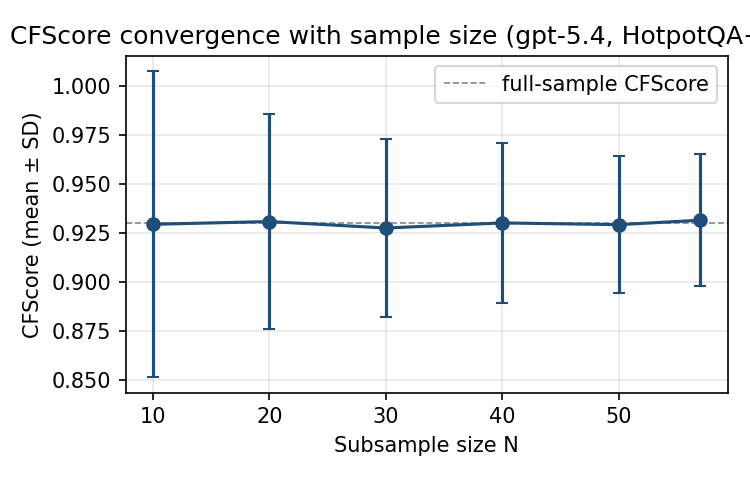
\includegraphics[width=\columnwidth]{figures/bootstrap_convergence.png}
    \caption{Bootstrap subsample convergence of the headline CFScore (1{,}000 random subsets per $N$). The mean is constant at $0.929$--$0.931$ and the SD falls from $0.078$ ($N{=}10$) to $0.034$ ($N{=}57$), flattening beyond $N{\approx}40$.}
    \label{fig:bootstrap}
\end{figure}

\label{app:bootstrap}
10,000-resample bootstrap on the headline CFScore: mean 0.930, 95\% percentile CI $[0.860, 0.982]$; leave-one-out influence bounded by $\pm 0.017$; subsample convergence SD falls from 0.078 ($N{=}10$) to 0.034 ($N{=}57$).

\section{Selection-Bias Robustness}
\label{app:selection}
Three abstention policies: exclude (headline, $+0.657$); abstention$\to$no-flip ($+0.329$); abstention$\to$flip-on-both ($+0.329$). The most conservative policy remains positive.

\section{Content-Matched Control}
\label{app:content}
BGE top-$k$ most-similar-to-gold deletion: $\widehat{F_R}$ 31.0\%$\to$38.3\%, CFScore $+0.557\to+0.483$, gap $48.4$pp. Matching diagnostics: length 22.3 vs 22.8 words; position 0.472 vs 0.473; question-word overlap 0.312 vs 0.274.

\section{2D Stratification}
\label{app:2d}
Valid\&sensitive 185q (AUROC 0.762); valid\&insensitive 19q (0.085); invalid\&sensitive 54q (0.683); invalid\&insensitive 42q (0.465).

\section{Merged-Prompt Variants}
\label{app:merged}
Full three-variant ablation on Mistral-7B and the GPT-5.4 comparison (see Table~4 of the LNCS version; numbers reproduced in the supplementary results JSON).

\section{Random-Baseline Sample Count}
\label{app:kablation}
We test how $K$ (random-baseline sample count) affects stability on Mistral-7B. The $K$-ablation confirms the variance analysis $\mathrm{Var}(\widehat{F_R}) = F_R(1-F_R)/(NK)$: $\widehat{F_T}$ is invariant in $K$ ($87.5\%$ at $K{=}1,3,5$) while $\widehat{F_R}$ sharpens from $31.2\%$ to $22.5\%$, lifting CFScore from $+0.562$ to $+0.650$. $K{=}1$ suffices when the random baseline is small (the GPT-5.4 regime); $K \in \{3,5\}$ is worth the extra calls on noisier models (App.~\ref{app:kablation}).

\section{Semantic-Distance Delta}
\label{app:semantic}
BGE cosine-distance $\Delta$ under 5-fold CV: semantic CFScore F1 $0.759{\pm}0.027$ vs exact-match $0.692{\pm}0.047$.

\end{document}